\section{Current-debt finance and creditor inheritance}
\label{sec:finance}

\subsection{Payable debt, genuine insolvency and inaccessible assets}

The sixty eliminations include fifty-six declarations and four automatic terminations. In fifty-six cases, the current debt exceeds the generous own-asset bound in Equation~\ref{eq:bound}: the player's own sales and mortgages cannot pay. Of the remaining four, three have legal payment routes and one is blocked by the implemented liquidation menu despite sufficient nominal assets (Figure~\ref{fig:finance}).

\begin{figure}[H]
\centering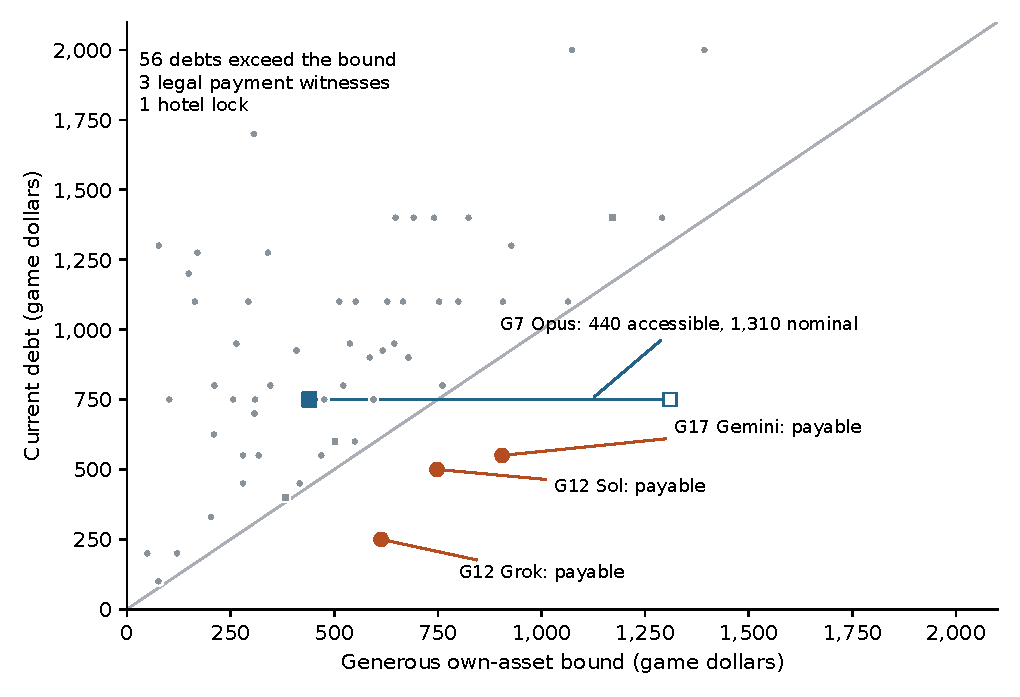
\includegraphics[width=0.9\linewidth]{finance.pdf}
\caption{Debt and the generous own-asset bound at all sixty eliminations. Points above the diagonal exceed the bound. The G7 segment separates nominal resources (1,310) from reachable cash (440) against a debt of 750. Squares mark the four automatic eliminations; G7 has a filled reachable-cash marker and a hollow nominal-bound marker. Payment witnesses concern the current debt.}
\label{fig:finance}
\end{figure}

The payable cases have distinct evidence. Sol's G12 d190 and Gemini's G17 d234 accounts omit collateral unlocked by building sales. Retained witnesses pay debts of \$500 and \$550 and leave \$38 and \$180 respectively. Cash plus immediately mortgageable deeds falls short in both, but that subtotal is not the entire menu, which includes sales. The third case is a same-response conflict, shown below; it can be resolved by house sales alone.

G7 d339 shows why nominal assets and usable finance differ. Opus owes \$750, has \$390 and can mortgage Oriental for \$50. Its pinks have four houses, four houses and a hotel, while the bank has no houses. The sale menu lists only highest-built deeds and offers a hotel sale only when four bank houses can replace it. It therefore offers no sale action, only the Oriental mortgage and bankruptcy. The retained continuation reaches \$440 and automatic bankruptcy despite \$1,310 in nominal resources. This is a menu-level restriction; Appendix~\ref{app:rules} distinguishes it from the separate validator's broader treatment of bundled sales.

The record also shows correct financing and insolvency judgments. At G20 d327--336, Sol combines \$49 cash, \$700 building salvage and \$665 mortgages to pay a \$1,400 debt, leaving \$14. In G16, Gemini declares bankruptcy at the first debt menu with \$288. Its note correctly calculates that \$375 of building salvage and \$730 of mortgages would bring the total to only \$1,393 against a \$2,000 debt. The first is an executed payment sequence; the second is a correct calculation of an unpayable position.

\TranscriptTitle{g12}{A payable debt ends in contradictory execution}

At G12 d249, Grok owes \$250 and has \$43. Its pink group has two, two and three houses. Assistant content requests a Virginia sale:
\TranscriptQuote{g12-sale}
The attached private note concludes:
\TranscriptQuote{g12_d249_private_final}
The sole received tool call instead declares bankruptcy, with this public message:
\TranscriptQuote{g12_d249_public_bankruptcy}
\TranscriptFinding{The engine eliminates Grok without selling houses, transferring its estate to Opus. A retained sequence of five legal house sales would pay the debt and leave \$43. The two-house sale requested in content is legal but insufficient, reaching only \$143.}
\TranscriptReading{The private note initially calls payment impossible, then derives the five-sale route and its correct \$43 remainder, although it miscounts the houses left. The received call nevertheless declares bankruptcy, and its public message supports that action. This separates recognition of a payment route from its execution: the record contains the financing reasoning and an incompatible applied action.}
\TranscriptSource{G12 d249, standard attempt 0. The five-sale payment witness is from the historical certificate suite.}

The disagreement also occurs in the other direction. In seven other Grok records, content names bankruptcy while the received call mortgages a deed in five or sells buildings in two. Those financing actions are not necessarily sufficient to pay; their source records are retained in the archive.

\subsection{Estates redistribute groups while the game continues}

During continuing play, estates complete fifty-two groups, forty-five owned by eventual winners; eighteen of sixty-three trade-completed groups belong to eventual winners. The contrast describes concentration conditional on the same games' outcomes. Across all stable acquisition boundaries there are 209 episodes: sixteen through direct purchase, nine through auction, sixty-three through trade and 121 through inheritance. Sixty-nine inherited completions occur at the final elimination and provide no further management opportunity (Table~\ref{tab:routes}).

\begin{table}[t]
\centering\small
\begin{tabularx}{\linewidth}{@{}lrrY@{}}
\toprule
Completing acquisition & Episodes & Eventual winner & Further play\\
\midrule
Trade & 63 & 18 & All episodes have a management window\\
Direct purchase & 16 & 12 & Before game end\\
Auction & 9 & 2 & Before game end\\
Nonterminal estate & 52 & 45 & Play continues\\
Terminal estate & 69 & 69 & No later management or income\\
\bottomrule
\end{tabularx}
\caption{Completion routes and eventual owner outcomes. Winner status is determined by the same trajectory, so these columns describe concentration rather than an effect on victory. Inherited deeds can also contribute to groups completed later by another route.}
\label{tab:routes}
\end{table}

Trade transfers 207 deeds. Estates transfer 397, including 227 before the final elimination. Eventual winners receive 202 of those 227 nonterminal deeds and are creditors in 35 of forty nonterminal eliminations, compared with 54 of sixty overall. The eventual winner receives the first estate in eighteen games and all three estates in sixteen. In 57 of sixty eliminations, including 38 of forty nonterminal ones, the debt is rent on the creditor's developed color deed. An established rent-producing position can therefore be followed by further asset concentration through inheritance. These counts describe that sequence, not inheritance's separate contribution to victory.

Routes also differ in income and timing. Fifty-one of sixty-three trade-completed groups collect rent, totaling \$57,378 after completion; directly purchased completions collect \$23,070. Estate-completed groups collect \$11,472, with fourteen of fifty-two nonterminal episodes receiving any rent. Later acquisition leaves less exposure, and rent on inherited buildings need not involve new spending. Of fifty-eight winner spending units, thirty-four contain an inherited deed at first own expenditure, while only thirty first become complete through an estate. Four mixed-route units close through a later purchase or trade.

Two winners, Sol in G14 and Gemini in G15, settle no trade. Gemini's G15 orange group completes through a Tennessee purchase and receives its first build on turn 47. It later collects \$3,250 in developed orange rent. Oranges trigger the first two eliminations; inherited browns trigger the last. The green group completes only through the terminal estate. The trajectory connects an early bank purchase to rent income, creditor acquisitions and the final elimination.

\subsection{Negotiating over prospective estates}

The creditor rule gives every player a stake in a distressed opponent's fate. The next exchanges explicitly refer to that stake. They also show why a later trajectory cannot establish the success or sincerity of a prior pitch.

\TranscriptTitle{g13}{An insurance pitch omits an available mortgage}

At G13 turn 107, Grok has \$35, owns yellow and stands nine squares before Short Line, where Sol's four railroads charge \$200. Ventnor remains unmortgaged and is worth \$130 in mortgage cash. Grok offers its mortgaged Pennsylvania to Opus for \$200:
\TranscriptQuote{g13-opening-insurance}
Opus counters at \$130 and records a reason to keep Grok solvent. That account follows Grok's opening appeal; it is not an independently established motive preceding the seller's framing. Grok replies:
\TranscriptQuote{g13-seller-counter}
Its applied note recognizes the Ventnor route and sets a \$165 floor. Returned provider reasoning also states:
\TranscriptQuote{g13-omission-explanation}
Opus accepts:
\TranscriptQuote{g13-acceptance}
\TranscriptFinding{Opus pays \$200 and \$16 mortgage-transfer interest. Seven turns later it buys North Carolina at auction for \$650, completing its greens with the acquired Pennsylvania. In the retained conditional acceptance branch, \$130 plus Grok's \$35 and a later \$130 Ventnor mortgage gives \$295, enough for the threatened rent. Grok does not land on Short Line on its next roll. It later pays \$200 on B\&O at turn 146, leaving \$49, and goes bankrupt on Short Line at turn 150; the yellows pass to Sol.}
\TranscriptReading{Grok frames the sale as insurance against Sol inheriting its estate and expressly describes omitting available collateral in one returned explanation. Opus echoes the estate stakes and pays \$200, but does not affirm the claimed \$130 financing limit. The opening appeal also overstates the landing probability: Short Line is nine squares away, a 4/36 roll, not 5/36. The d252 explanation itself considers accepting \$130 before countering at \$200. The record shows selective disclosure, buyer uptake of the estate framing and a settled price, while leaving the cause of the \$70 difference unidentified. Later bankruptcy follows the actual trajectory; it does not measure survival time purchased by the deal.}
\TranscriptSource{G13 d250--253, d307 and d311; auction purchase event 1911. Grok uses standard responses; Opus uses action-only recovery, with provider explanations rather than applied private notes. The focal recipient requests contain the messages and a garbled history line, alongside correct holdings.}

\TranscriptTitle{g18}{A repeated price is withdrawn after the seller deteriorates}

Opus repeatedly offers \$250 for Sol's mortgaged Pacific, which would complete Opus's greens. After receiving \$750 rent from Sol, it repeats the assurance:
\TranscriptQuote{g18-assurance}
A second \$750 payment then forces Sol to sell orange buildings and mortgage its remaining red deeds, leaving \$49. After larger packages fail, Sol invokes the advertised price:
\TranscriptQuote{g18-invocation}
\TranscriptQuote{g18-withdrawal}
Opus's returned explanation supplies a reason:
\TranscriptQuote{g18-withdrawal-explanation}
\TranscriptFinding{No sale occurs at \$250. Opus redeems Pennsylvania at turn 190 and North Carolina at turn 192, then bids \$150 and \$225 for Pacific at turn 194. Sol asks \$450 and \$350 and later offers it at \$300; none settles. Opus eventually receives Sol's estate and wins. The earlier assurance is present in the requests at invocation and withdrawal.}
\TranscriptReading{The withdrawal changes the terms rather than ending interest in the group. Opus's explanation cites the cost of prolonging a nearly bankrupt rival and of developing greens, yet it redeems its two green deeds and resumes bidding below the withdrawn price. These actions document continued bargaining after the seller's financial deterioration. The standing offer is a public assurance without an engine-enforced commitment; the record identifies no costly action taken in reliance or dishonesty when the original assurance was made.}
\TranscriptSource{G18 d421--461. Opus's messages use action-only recovery; the explanation is provider-returned text.}
